\documentclass[1p]{elsarticle_modified}
%\bibliographystyle{elsarticle-num}

%\usepackage[colorlinks]{hyperref}
%\usepackage{abbrmath_seonhwa} %\Abb, \Ascr, \Acal ,\Abf, \Afrak
\usepackage{amsfonts}
\usepackage{amssymb}
\usepackage{amsmath}
\usepackage{amsthm}
\usepackage{scalefnt}
\usepackage{amsbsy}
\usepackage{kotex}
\usepackage{caption}
\usepackage{subfig}
\usepackage{color}
\usepackage{graphicx}
\usepackage{xcolor} %% white, black, red, green, blue, cyan, magenta, yellow
\usepackage{float}
\usepackage{setspace}
\usepackage{hyperref}

\usepackage{tikz}
\usetikzlibrary{arrows}

\usepackage{multirow}
\usepackage{array} % fixed length table
\usepackage{hhline}

%%%%%%%%%%%%%%%%%%%%%
\makeatletter
\renewcommand*\env@matrix[1][\arraystretch]{%
	\edef\arraystretch{#1}%
	\hskip -\arraycolsep
	\let\@ifnextchar\new@ifnextchar
	\array{*\c@MaxMatrixCols c}}
\makeatother %https://tex.stackexchange.com/questions/14071/how-can-i-increase-the-line-spacing-in-a-matrix
%%%%%%%%%%%%%%%

\usepackage[normalem]{ulem}

\newcommand{\msout}[1]{\ifmmode\text{\sout{\ensuremath{#1}}}\else\sout{#1}\fi}
%SOURCE: \msout is \stkout macro in https://tex.stackexchange.com/questions/20609/strikeout-in-math-mode

\newcommand{\cancel}[1]{
	\ifmmode
	{\color{red}\msout{#1}}
	\else
	{\color{red}\sout{#1}}
	\fi
}

\newcommand{\add}[1]{
	{\color{blue}\uwave{#1}}
}

\newcommand{\replace}[2]{
	\ifmmode
	{\color{red}\msout{#1}}{\color{blue}\uwave{#2}}
	\else
	{\color{red}\sout{#1}}{\color{blue}\uwave{#2}}
	\fi
}

\newcommand{\Sol}{\mathcal{S}} %segment
\newcommand{\D}{D} %diagram
\newcommand{\A}{\mathcal{A}} %arc


%%%%%%%%%%%%%%%%%%%%%%%%%%%%%5 test

\def\sl{\operatorname{\textup{SL}}(2,\Cbb)}
\def\psl{\operatorname{\textup{PSL}}(2,\Cbb)}
\def\quan{\mkern 1mu \triangleright \mkern 1mu}

\theoremstyle{definition}
\newtheorem{thm}{Theorem}[section]
\newtheorem{prop}[thm]{Proposition}
\newtheorem{lem}[thm]{Lemma}
\newtheorem{ques}[thm]{Question}
\newtheorem{cor}[thm]{Corollary}
\newtheorem{defn}[thm]{Definition}
\newtheorem{exam}[thm]{Example}
\newtheorem{rmk}[thm]{Remark}
\newtheorem{alg}[thm]{Algorithm}

\newcommand{\I}{\sqrt{-1}}
\begin{document}

%\begin{frontmatter}
%
%\title{Boundary parabolic representations of knots up to 8 crossings}
%
%%% Group authors per affiliation:
%\author{Yunhi Cho} 
%\address{Department of Mathematics, University of Seoul, Seoul, Korea}
%\ead{yhcho@uos.ac.kr}
%
%
%\author{Seonhwa Kim} %\fnref{s_kim}}
%\address{Center for Geometry and Physics, Institute for Basic Science, Pohang, 37673, Korea}
%\ead{ryeona17@ibs.re.kr}
%
%\author{Hyuk Kim}
%\address{Department of Mathematical Sciences, Seoul National University, Seoul 08826, Korea}
%\ead{hyukkim@snu.ac.kr}
%
%\author{Seokbeom Yoon}
%\address{Department of Mathematical Sciences, Seoul National University, Seoul, 08826,  Korea}
%\ead{sbyoon15@snu.ac.kr}
%
%\begin{abstract}
%We find all boundary parabolic representation of knots up to 8 crossings.
%
%\end{abstract}
%\begin{keyword}
%    \MSC[2010] 57M25 
%\end{keyword}
%
%\end{frontmatter}

%\linenumbers
%\tableofcontents
%
\newcommand\colored[1]{\textcolor{white}{\rule[-0.35ex]{0.8em}{1.4ex}}\kern-0.8em\color{red} #1}%
%\newcommand\colored[1]{\textcolor{white}{ #1}\kern-2.17ex	\textcolor{white}{ #1}\kern-1.81ex	\textcolor{white}{ #1}\kern-2.15ex\color{red}#1	}

{\Large $\underline{12n_{0306}~(K12n_{0306})}$}

\setlength{\tabcolsep}{10pt}
\renewcommand{\arraystretch}{1.6}
\vspace{1cm}\begin{tabular}{m{100pt}>{\centering\arraybackslash}m{274pt}}
\multirow{5}{120pt}{
	\centering
	\includegraphics[width=112pt]{../../../GIT/diagram.site/Diagrams/png/2395_12n_0306.png}\\
\ \ \ A knot diagram\footnotemark}&
\allowdisplaybreaks
\textbf{Linearized knot diagam} \\
\cline{2-2}
 &
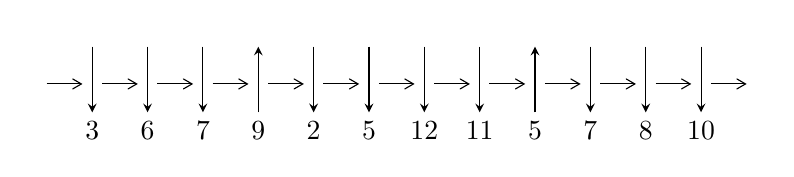
\begin{tikzpicture}[x=20pt, y=17pt]
	% nodes
	\node (C0) at (0, 0) {};
	\node (C1) at (1, 0) {};
	\node (C1U) at (1, +1) {};
	\node (C1D) at (1, -1) {3};

	\node (C2) at (2, 0) {};
	\node (C2U) at (2, +1) {};
	\node (C2D) at (2, -1) {6};

	\node (C3) at (3, 0) {};
	\node (C3U) at (3, +1) {};
	\node (C3D) at (3, -1) {7};

	\node (C4) at (4, 0) {};
	\node (C4U) at (4, +1) {};
	\node (C4D) at (4, -1) {9};

	\node (C5) at (5, 0) {};
	\node (C5U) at (5, +1) {};
	\node (C5D) at (5, -1) {2};

	\node (C6) at (6, 0) {};
	\node (C6U) at (6, +1) {};
	\node (C6D) at (6, -1) {5};

	\node (C7) at (7, 0) {};
	\node (C7U) at (7, +1) {};
	\node (C7D) at (7, -1) {12};

	\node (C8) at (8, 0) {};
	\node (C8U) at (8, +1) {};
	\node (C8D) at (8, -1) {11};

	\node (C9) at (9, 0) {};
	\node (C9U) at (9, +1) {};
	\node (C9D) at (9, -1) {5};

	\node (C10) at (10, 0) {};
	\node (C10U) at (10, +1) {};
	\node (C10D) at (10, -1) {7};

	\node (C11) at (11, 0) {};
	\node (C11U) at (11, +1) {};
	\node (C11D) at (11, -1) {8};

	\node (C12) at (12, 0) {};
	\node (C12U) at (12, +1) {};
	\node (C12D) at (12, -1) {10};
	\node (C13) at (13, 0) {};

	% arrows
	\draw[->,>={angle 60}]
	(C0) edge (C1) (C1) edge (C2) (C2) edge (C3) (C3) edge (C4) (C4) edge (C5) (C5) edge (C6) (C6) edge (C7) (C7) edge (C8) (C8) edge (C9) (C9) edge (C10) (C10) edge (C11) (C11) edge (C12) (C12) edge (C13) ;	\draw[->,>=stealth]
	(C1U) edge (C1D) (C2U) edge (C2D) (C3U) edge (C3D) (C4D) edge (C4U) (C5U) edge (C5D) (C6U) edge (C6D) (C7U) edge (C7D) (C8U) edge (C8D) (C9D) edge (C9U) (C10U) edge (C10D) (C11U) edge (C11D) (C12U) edge (C12D) ;
	\end{tikzpicture} \\
\hhline{~~} \\& 
\textbf{Solving Sequence} \\ \cline{2-2} 
 &
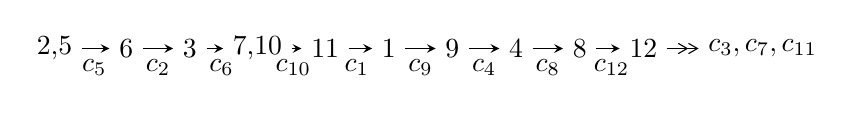
\begin{tikzpicture}[x=23pt, y=7pt]
	% node
	\node (A0) at (-1/8, 0) {2,5};
	\node (A1) at (1, 0) {6};
	\node (A2) at (2, 0) {3};
	\node (A3) at (49/16, 0) {7,10};
	\node (A4) at (33/8, 0) {11};
	\node (A5) at (41/8, 0) {1};
	\node (A6) at (49/8, 0) {9};
	\node (A7) at (57/8, 0) {4};
	\node (A8) at (65/8, 0) {8};
	\node (A9) at (73/8, 0) {12};
	\node (C1) at (1/2, -1) {$c_{5}$};
	\node (C2) at (3/2, -1) {$c_{2}$};
	\node (C3) at (5/2, -1) {$c_{6}$};
	\node (C4) at (29/8, -1) {$c_{10}$};
	\node (C5) at (37/8, -1) {$c_{1}$};
	\node (C6) at (45/8, -1) {$c_{9}$};
	\node (C7) at (53/8, -1) {$c_{4}$};
	\node (C8) at (61/8, -1) {$c_{8}$};
	\node (C9) at (69/8, -1) {$c_{12}$};
	\node (A10) at (11, 0) {$c_{3},c_{7},c_{11}$};

	% edge
	\draw[->,>=stealth]	
	(A0) edge (A1) (A1) edge (A2) (A2) edge (A3) (A3) edge (A4) (A4) edge (A5) (A5) edge (A6) (A6) edge (A7) (A7) edge (A8) (A8) edge (A9) ;
	\draw[->>,>={angle 60}]	
	(A9) edge (A10);
\end{tikzpicture} \\ 

\end{tabular} \\

\footnotetext{
The image of knot diagram is generated by the software ``\textbf{Draw programme}" developed by Andrew Bartholomew(\url{http://www.layer8.co.uk/maths/draw/index.htm\#Running-draw}), where we modified some parts for our purpose(\url{https://github.com/CATsTAILs/LinksPainter}).
}\phantom \\ \newline 
\centering \textbf{Ideals for irreducible components\footnotemark of $X_{\text{par}}$} 
 
\begin{align*}
I^u_{1}&=\langle 
-3 u^{25}-12 u^{24}+\cdots+2 b+3,\;u^{25}+10 u^{24}+\cdots+4 a+11,\;u^{26}+4 u^{25}+\cdots- u-1\rangle \\
I^u_{2}&=\langle 
b,\;u^2+a- u,\;u^3- u^2+1\rangle \\
I^u_{3}&=\langle 
b,\;- u^2 a+a^2+2 a u+u^2- a-2 u+2,\;u^3- u^2+1\rangle \\
\\
\end{align*}
\raggedright * 3 irreducible components of $\dim_{\mathbb{C}}=0$, with total 35 representations.\\
\footnotetext{All coefficients of polynomials are rational numbers. But the coefficients are sometimes approximated in decimal forms when there is not enough margin.}
\newpage
\renewcommand{\arraystretch}{1}
\centering \section*{I. $I^u_{1}= \langle -3 u^{25}-12 u^{24}+\cdots+2 b+3,\;u^{25}+10 u^{24}+\cdots+4 a+11,\;u^{26}+4 u^{25}+\cdots- u-1 \rangle$}
\flushleft \textbf{(i) Arc colorings}\\
\begin{tabular}{m{7pt} m{180pt} m{7pt} m{180pt} }
\flushright $a_{2}=$&$\begin{pmatrix}0\\u\end{pmatrix}$ \\
\flushright $a_{5}=$&$\begin{pmatrix}1\\0\end{pmatrix}$ \\
\flushright $a_{6}=$&$\begin{pmatrix}1\\u^2\end{pmatrix}$ \\
\flushright $a_{3}=$&$\begin{pmatrix}- u\\- u^3+u\end{pmatrix}$ \\
\flushright $a_{7}=$&$\begin{pmatrix}- u^2+1\\u^2\end{pmatrix}$ \\
\flushright $a_{10}=$&$\begin{pmatrix}-\frac{1}{4} u^{25}-\frac{5}{2} u^{24}+\cdots-\frac{13}{2} u-\frac{11}{4}\\\frac{3}{2} u^{25}+6 u^{24}+\cdots+u-\frac{3}{2}\end{pmatrix}$ \\
\flushright $a_{11}=$&$\begin{pmatrix}-\frac{1}{2} u^{25}-\frac{9}{4} u^{24}+\cdots-\frac{15}{2} u-\frac{17}{4}\\\frac{1}{4} u^{24}+\frac{5}{4} u^{23}+\cdots+\frac{7}{4} u^2+\frac{3}{4} u\end{pmatrix}$ \\
\flushright $a_{1}=$&$\begin{pmatrix}u^3\\u^5- u^3+u\end{pmatrix}$ \\
\flushright $a_{9}=$&$\begin{pmatrix}-\frac{7}{4} u^{25}-\frac{17}{2} u^{24}+\cdots-\frac{15}{2} u-\frac{5}{4}\\\frac{3}{2} u^{25}+6 u^{24}+\cdots+u-\frac{3}{2}\end{pmatrix}$ \\
\flushright $a_{4}=$&$\begin{pmatrix}u^7-2 u^5+2 u^3-2 u\\- u^7+u^5-2 u^3+u\end{pmatrix}$ \\
\flushright $a_{8}=$&$\begin{pmatrix}-\frac{3}{4} u^{25}-\frac{13}{4} u^{24}+\cdots-\frac{7}{4} u+\frac{1}{4}\\\frac{1}{4} u^{25}+u^{24}+\cdots+3 u^2-\frac{1}{4}\end{pmatrix}$ \\
\flushright $a_{12}=$&$\begin{pmatrix}\frac{1}{4} u^{23}+\frac{3}{4} u^{22}+\cdots+\frac{9}{4} u+\frac{5}{4}\\- u^2\end{pmatrix}$\\&\end{tabular}
\flushleft \textbf{(ii) Obstruction class $= -1$}\\~\\
\flushleft \textbf{(iii) Cusp Shapes $= \frac{11}{4} u^{25}+\frac{21}{2} u^{24}+\cdots+\frac{17}{4} u-\frac{35}{2}$}\\~\\
\newpage\renewcommand{\arraystretch}{1}
\flushleft \textbf{(iv) u-Polynomials at the component}\newline \\
\begin{tabular}{m{50pt}|m{274pt}}
Crossings & \hspace{64pt}u-Polynomials at each crossing \\
\hline $$\begin{aligned}c_{1},c_{6}\end{aligned}$$&$\begin{aligned}
&u^{26}+4 u^{25}+\cdots+15 u+1
\end{aligned}$\\
\hline $$\begin{aligned}c_{2},c_{5}\end{aligned}$$&$\begin{aligned}
&u^{26}+4 u^{25}+\cdots- u-1
\end{aligned}$\\
\hline $$\begin{aligned}c_{3}\end{aligned}$$&$\begin{aligned}
&u^{26}-4 u^{25}+\cdots-103464 u-31428
\end{aligned}$\\
\hline $$\begin{aligned}c_{4},c_{9}\end{aligned}$$&$\begin{aligned}
&u^{26}- u^{25}+\cdots-3456 u^2+512
\end{aligned}$\\
\hline $$\begin{aligned}c_{7},c_{8},c_{11}\end{aligned}$$&$\begin{aligned}
&u^{26}-4 u^{25}+\cdots+7 u-1
\end{aligned}$\\
\hline $$\begin{aligned}c_{10}\end{aligned}$$&$\begin{aligned}
&u^{26}+4 u^{25}+\cdots+889 u-193
\end{aligned}$\\
\hline $$\begin{aligned}c_{12}\end{aligned}$$&$\begin{aligned}
&u^{26}+28 u^{24}+\cdots+25 u+3
\end{aligned}$\\
\hline
\end{tabular}\\~\\
\newpage\renewcommand{\arraystretch}{1}
\flushleft \textbf{(v) Riley Polynomials at the component}\newline \\
\begin{tabular}{m{50pt}|m{274pt}}
Crossings & \hspace{64pt}Riley Polynomials at each crossing \\
\hline $$\begin{aligned}c_{1},c_{6}\end{aligned}$$&$\begin{aligned}
&y^{26}+40 y^{25}+\cdots-15 y+1
\end{aligned}$\\
\hline $$\begin{aligned}c_{2},c_{5}\end{aligned}$$&$\begin{aligned}
&y^{26}-4 y^{25}+\cdots-15 y+1
\end{aligned}$\\
\hline $$\begin{aligned}c_{3}\end{aligned}$$&$\begin{aligned}
&y^{26}+124 y^{25}+\cdots-27391370184 y+987719184
\end{aligned}$\\
\hline $$\begin{aligned}c_{4},c_{9}\end{aligned}$$&$\begin{aligned}
&y^{26}-49 y^{25}+\cdots-3538944 y+262144
\end{aligned}$\\
\hline $$\begin{aligned}c_{7},c_{8},c_{11}\end{aligned}$$&$\begin{aligned}
&y^{26}+28 y^{25}+\cdots-23 y+1
\end{aligned}$\\
\hline $$\begin{aligned}c_{10}\end{aligned}$$&$\begin{aligned}
&y^{26}+28 y^{25}+\cdots-417831 y+37249
\end{aligned}$\\
\hline $$\begin{aligned}c_{12}\end{aligned}$$&$\begin{aligned}
&y^{26}+56 y^{25}+\cdots-1231 y+9
\end{aligned}$\\
\hline
\end{tabular}\\~\\
\newpage\flushleft \textbf{(vi) Complex Volumes and Cusp Shapes}
$$\begin{array}{c|c|c}  
\text{Solutions to }I^u_{1}& \I (\text{vol} + \sqrt{-1}CS) & \text{Cusp shape}\\
 \hline 
\begin{aligned}
u &= -0.927978 + 0.281302 I \\
a &= -0.892022 + 0.688694 I \\
b &= -0.624177 + 0.789814 I\end{aligned}
 & \phantom{-}2.80822 + 0.17134 I & -6.35112 - 1.45434 I \\ \hline\begin{aligned}
u &= -0.927978 - 0.281302 I \\
a &= -0.892022 - 0.688694 I \\
b &= -0.624177 - 0.789814 I\end{aligned}
 & \phantom{-}2.80822 - 0.17134 I & -6.35112 + 1.45434 I \\ \hline\begin{aligned}
u &= \phantom{-}0.736454 + 0.746707 I \\
a &= \phantom{-}0.855774 + 0.275171 I \\
b &= -0.860539 + 0.488199 I\end{aligned}
 & \phantom{-}3.28913 - 1.44124 I & -2.49548 + 1.39542 I \\ \hline\begin{aligned}
u &= \phantom{-}0.736454 - 0.746707 I \\
a &= \phantom{-}0.855774 - 0.275171 I \\
b &= -0.860539 - 0.488199 I\end{aligned}
 & \phantom{-}3.28913 + 1.44124 I & -2.49548 - 1.39542 I \\ \hline\begin{aligned}
u &= \phantom{-}0.930739 + 0.665116 I \\
a &= -0.109280 - 0.822401 I \\
b &= \phantom{-}0.882348 + 0.149927 I\end{aligned}
 & \phantom{-}2.63703 - 3.89810 I & -3.35232 + 6.23910 I \\ \hline\begin{aligned}
u &= \phantom{-}0.930739 - 0.665116 I \\
a &= -0.109280 + 0.822401 I \\
b &= \phantom{-}0.882348 - 0.149927 I\end{aligned}
 & \phantom{-}2.63703 + 3.89810 I & -3.35232 - 6.23910 I \\ \hline\begin{aligned}
u &= -0.828014\phantom{ +0.000000I} \\
a &= \phantom{-}0.505037\phantom{ +0.000000I} \\
b &= \phantom{-}0.430120\phantom{ +0.000000I}\end{aligned}
 & -1.35925\phantom{ +0.000000I} & -5.94650\phantom{ +0.000000I} \\ \hline\begin{aligned}
u &= \phantom{-}0.670758 + 0.970438 I \\
a &= -1.198940 - 0.023490 I \\
b &= \phantom{-}1.59537 - 1.11430 I\end{aligned}
 & \phantom{-}10.51200 - 0.45901 I & -0.702444 + 1.109804 I \\ \hline\begin{aligned}
u &= \phantom{-}0.670758 - 0.970438 I \\
a &= -1.198940 + 0.023490 I \\
b &= \phantom{-}1.59537 + 1.11430 I\end{aligned}
 & \phantom{-}10.51200 + 0.45901 I & -0.702444 - 1.109804 I \\ \hline\begin{aligned}
u &= -0.437740 + 0.645989 I \\
a &= -0.332493 + 0.449600 I \\
b &= \phantom{-}0.029303 + 1.123950 I\end{aligned}
 & \phantom{-}4.72486 + 3.33852 I & -2.36603 - 3.49962 I\\
 \hline 
 \end{array}$$\newpage$$\begin{array}{c|c|c}  
\text{Solutions to }I^u_{1}& \I (\text{vol} + \sqrt{-1}CS) & \text{Cusp shape}\\
 \hline 
\begin{aligned}
u &= -0.437740 - 0.645989 I \\
a &= -0.332493 - 0.449600 I \\
b &= \phantom{-}0.029303 - 1.123950 I\end{aligned}
 & \phantom{-}4.72486 - 3.33852 I & -2.36603 + 3.49962 I \\ \hline\begin{aligned}
u &= \phantom{-}1.079900 + 0.695708 I \\
a &= -0.362002 + 1.203280 I \\
b &= -1.56097 - 0.59580 I\end{aligned}
 & \phantom{-}9.04679 - 5.69366 I & -2.13177 + 3.88502 I \\ \hline\begin{aligned}
u &= \phantom{-}1.079900 - 0.695708 I \\
a &= -0.362002 - 1.203280 I \\
b &= -1.56097 + 0.59580 I\end{aligned}
 & \phantom{-}9.04679 + 5.69366 I & -2.13177 - 3.88502 I \\ \hline\begin{aligned}
u &= -0.953135 + 0.981373 I \\
a &= \phantom{-}1.41685 - 1.08331 I \\
b &= -2.31682 + 0.09546 I\end{aligned}
 & \phantom{-}14.7661 + 0.7496 I & -4.35446 + 0.19083 I \\ \hline\begin{aligned}
u &= -0.953135 - 0.981373 I \\
a &= \phantom{-}1.41685 + 1.08331 I \\
b &= -2.31682 - 0.09546 I\end{aligned}
 & \phantom{-}14.7661 - 0.7496 I & -4.35446 - 0.19083 I \\ \hline\begin{aligned}
u &= -0.996483 + 0.952652 I \\
a &= -1.54076 + 1.18418 I \\
b &= \phantom{-}2.26473 + 0.34444 I\end{aligned}
 & \phantom{-}14.6174 + 6.3423 I & -4.67499 - 4.46303 I \\ \hline\begin{aligned}
u &= -0.996483 - 0.952652 I \\
a &= -1.54076 - 1.18418 I \\
b &= \phantom{-}2.26473 - 0.34444 I\end{aligned}
 & \phantom{-}14.6174 - 6.3423 I & -4.67499 + 4.46303 I \\ \hline\begin{aligned}
u &= -0.918139 + 1.031730 I \\
a &= -1.21694 + 1.06831 I \\
b &= \phantom{-}2.52632 - 0.56908 I\end{aligned}
 & -17.5237 - 3.4354 I & -1.66037 + 0.61088 I \\ \hline\begin{aligned}
u &= -0.918139 - 1.031730 I \\
a &= -1.21694 - 1.06831 I \\
b &= \phantom{-}2.52632 + 0.56908 I\end{aligned}
 & -17.5237 + 3.4354 I & -1.66037 - 0.61088 I \\ \hline\begin{aligned}
u &= -1.046110 + 0.939916 I \\
a &= \phantom{-}1.58869 - 1.30078 I \\
b &= -2.33420 - 0.78739 I\end{aligned}
 & -17.9709 + 10.6421 I & -2.17770 - 4.87168 I\\
 \hline 
 \end{array}$$\newpage$$\begin{array}{c|c|c}  
\text{Solutions to }I^u_{1}& \I (\text{vol} + \sqrt{-1}CS) & \text{Cusp shape}\\
 \hline 
\begin{aligned}
u &= -1.046110 - 0.939916 I \\
a &= \phantom{-}1.58869 + 1.30078 I \\
b &= -2.33420 + 0.78739 I\end{aligned}
 & -17.9709 - 10.6421 I & -2.17770 + 4.87168 I \\ \hline\begin{aligned}
u &= \phantom{-}0.547038 + 0.202189 I \\
a &= \phantom{-}2.44519 + 0.75423 I \\
b &= -0.603638 + 0.076459 I\end{aligned}
 & \phantom{-}2.36049 - 3.21762 I & \phantom{-}0.10564 + 7.29080 I \\ \hline\begin{aligned}
u &= \phantom{-}0.547038 - 0.202189 I \\
a &= \phantom{-}2.44519 - 0.75423 I \\
b &= -0.603638 - 0.076459 I\end{aligned}
 & \phantom{-}2.36049 + 3.21762 I & \phantom{-}0.10564 - 7.29080 I \\ \hline\begin{aligned}
u &= -0.482360 + 0.313885 I \\
a &= \phantom{-}0.443368 - 0.835553 I \\
b &= \phantom{-}0.021358 - 0.703916 I\end{aligned}
 & -0.662371 + 1.026000 I & -7.80706 - 6.48797 I \\ \hline\begin{aligned}
u &= -0.482360 - 0.313885 I \\
a &= \phantom{-}0.443368 + 0.835553 I \\
b &= \phantom{-}0.021358 + 0.703916 I\end{aligned}
 & -0.662371 - 1.026000 I & -7.80706 + 6.48797 I \\ \hline\begin{aligned}
u &= \phantom{-}0.422126\phantom{ +0.000000I} \\
a &= -2.69989\phantom{ +0.000000I} \\
b &= \phantom{-}0.531699\phantom{ +0.000000I}\end{aligned}
 & -1.56806\phantom{ +0.000000I} & -4.11730\phantom{ +0.000000I}\\
 \hline 
 \end{array}$$\newpage\newpage\renewcommand{\arraystretch}{1}
\centering \section*{II. $I^u_{2}= \langle b,\;u^2+a- u,\;u^3- u^2+1 \rangle$}
\flushleft \textbf{(i) Arc colorings}\\
\begin{tabular}{m{7pt} m{180pt} m{7pt} m{180pt} }
\flushright $a_{2}=$&$\begin{pmatrix}0\\u\end{pmatrix}$ \\
\flushright $a_{5}=$&$\begin{pmatrix}1\\0\end{pmatrix}$ \\
\flushright $a_{6}=$&$\begin{pmatrix}1\\u^2\end{pmatrix}$ \\
\flushright $a_{3}=$&$\begin{pmatrix}- u\\- u^2+u+1\end{pmatrix}$ \\
\flushright $a_{7}=$&$\begin{pmatrix}- u^2+1\\u^2\end{pmatrix}$ \\
\flushright $a_{10}=$&$\begin{pmatrix}- u^2+u\\0\end{pmatrix}$ \\
\flushright $a_{11}=$&$\begin{pmatrix}-2 u^2+2 u+1\\u^2-1\end{pmatrix}$ \\
\flushright $a_{1}=$&$\begin{pmatrix}u^2-1\\- u^2\end{pmatrix}$ \\
\flushright $a_{9}=$&$\begin{pmatrix}- u^2+u\\0\end{pmatrix}$ \\
\flushright $a_{4}=$&$\begin{pmatrix}1\\0\end{pmatrix}$ \\
\flushright $a_{8}=$&$\begin{pmatrix}-2 u^2- u\\u+1\end{pmatrix}$ \\
\flushright $a_{12}=$&$\begin{pmatrix}u^2-2\\- u^2\end{pmatrix}$\\&\end{tabular}
\flushleft \textbf{(ii) Obstruction class $= 1$}\\~\\
\flushleft \textbf{(iii) Cusp Shapes $= - u^2+9 u-11$}\\~\\
\newpage\renewcommand{\arraystretch}{1}
\flushleft \textbf{(iv) u-Polynomials at the component}\newline \\
\begin{tabular}{m{50pt}|m{274pt}}
Crossings & \hspace{64pt}u-Polynomials at each crossing \\
\hline $$\begin{aligned}c_{1},c_{3},c_{7}\\c_{8}\end{aligned}$$&$\begin{aligned}
&u^3- u^2+2 u-1
\end{aligned}$\\
\hline $$\begin{aligned}c_{2}\end{aligned}$$&$\begin{aligned}
&u^3+u^2-1
\end{aligned}$\\
\hline $$\begin{aligned}c_{4},c_{9}\end{aligned}$$&$\begin{aligned}
&u^3
\end{aligned}$\\
\hline $$\begin{aligned}c_{5},c_{10},c_{12}\end{aligned}$$&$\begin{aligned}
&u^3- u^2+1
\end{aligned}$\\
\hline $$\begin{aligned}c_{6},c_{11}\end{aligned}$$&$\begin{aligned}
&u^3+u^2+2 u+1
\end{aligned}$\\
\hline
\end{tabular}\\~\\
\newpage\renewcommand{\arraystretch}{1}
\flushleft \textbf{(v) Riley Polynomials at the component}\newline \\
\begin{tabular}{m{50pt}|m{274pt}}
Crossings & \hspace{64pt}Riley Polynomials at each crossing \\
\hline $$\begin{aligned}c_{1},c_{3},c_{6}\\c_{7},c_{8},c_{11}\end{aligned}$$&$\begin{aligned}
&y^3+3 y^2+2 y-1
\end{aligned}$\\
\hline $$\begin{aligned}c_{2},c_{5},c_{10}\\c_{12}\end{aligned}$$&$\begin{aligned}
&y^3- y^2+2 y-1
\end{aligned}$\\
\hline $$\begin{aligned}c_{4},c_{9}\end{aligned}$$&$\begin{aligned}
&y^3
\end{aligned}$\\
\hline
\end{tabular}\\~\\
\newpage\flushleft \textbf{(vi) Complex Volumes and Cusp Shapes}
$$\begin{array}{c|c|c}  
\text{Solutions to }I^u_{2}& \I (\text{vol} + \sqrt{-1}CS) & \text{Cusp shape}\\
 \hline 
\begin{aligned}
u &= \phantom{-}0.877439 + 0.744862 I \\
a &= \phantom{-}0.662359 - 0.562280 I \\
b &= \phantom{-0.000000 } 0\end{aligned}
 & \phantom{-}6.04826 - 5.65624 I & -3.31813 + 5.39661 I \\ \hline\begin{aligned}
u &= \phantom{-}0.877439 - 0.744862 I \\
a &= \phantom{-}0.662359 + 0.562280 I \\
b &= \phantom{-0.000000 } 0\end{aligned}
 & \phantom{-}6.04826 + 5.65624 I & -3.31813 - 5.39661 I \\ \hline\begin{aligned}
u &= -0.754878\phantom{ +0.000000I} \\
a &= -1.32472\phantom{ +0.000000I} \\
b &= \phantom{-0.000000 } 0\end{aligned}
 & -2.22691\phantom{ +0.000000I} & -18.3640\phantom{ +0.000000I}\\
 \hline 
 \end{array}$$\newpage\newpage\renewcommand{\arraystretch}{1}
\centering \section*{III. $I^u_{3}= \langle b,\;- u^2 a+a^2+2 a u+u^2- a-2 u+2,\;u^3- u^2+1 \rangle$}
\flushleft \textbf{(i) Arc colorings}\\
\begin{tabular}{m{7pt} m{180pt} m{7pt} m{180pt} }
\flushright $a_{2}=$&$\begin{pmatrix}0\\u\end{pmatrix}$ \\
\flushright $a_{5}=$&$\begin{pmatrix}1\\0\end{pmatrix}$ \\
\flushright $a_{6}=$&$\begin{pmatrix}1\\u^2\end{pmatrix}$ \\
\flushright $a_{3}=$&$\begin{pmatrix}- u\\- u^2+u+1\end{pmatrix}$ \\
\flushright $a_{7}=$&$\begin{pmatrix}- u^2+1\\u^2\end{pmatrix}$ \\
\flushright $a_{10}=$&$\begin{pmatrix}a\\0\end{pmatrix}$ \\
\flushright $a_{11}=$&$\begin{pmatrix}a u+2 a\\u^2 a- a u- a\end{pmatrix}$ \\
\flushright $a_{1}=$&$\begin{pmatrix}u^2-1\\- u^2\end{pmatrix}$ \\
\flushright $a_{9}=$&$\begin{pmatrix}a\\0\end{pmatrix}$ \\
\flushright $a_{4}=$&$\begin{pmatrix}1\\0\end{pmatrix}$ \\
\flushright $a_{8}=$&$\begin{pmatrix}u^2 a+a u+u^2- a-2 u+3\\- u^2 a+u^2- u\end{pmatrix}$ \\
\flushright $a_{12}=$&$\begin{pmatrix}a u+2 u^2- a- u\\- u^2\end{pmatrix}$\\&\end{tabular}
\flushleft \textbf{(ii) Obstruction class $= 1$}\\~\\
\flushleft \textbf{(iii) Cusp Shapes $= 2 u^2 a+a u- a+3 u-7$}\\~\\
\newpage\renewcommand{\arraystretch}{1}
\flushleft \textbf{(iv) u-Polynomials at the component}\newline \\
\begin{tabular}{m{50pt}|m{274pt}}
Crossings & \hspace{64pt}u-Polynomials at each crossing \\
\hline $$\begin{aligned}c_{1},c_{3},c_{7}\\c_{8}\end{aligned}$$&$\begin{aligned}
&(u^3- u^2+2 u-1)^2
\end{aligned}$\\
\hline $$\begin{aligned}c_{2}\end{aligned}$$&$\begin{aligned}
&(u^3+u^2-1)^2
\end{aligned}$\\
\hline $$\begin{aligned}c_{4},c_{9}\end{aligned}$$&$\begin{aligned}
&u^6
\end{aligned}$\\
\hline $$\begin{aligned}c_{5},c_{10},c_{12}\end{aligned}$$&$\begin{aligned}
&(u^3- u^2+1)^2
\end{aligned}$\\
\hline $$\begin{aligned}c_{6},c_{11}\end{aligned}$$&$\begin{aligned}
&(u^3+u^2+2 u+1)^2
\end{aligned}$\\
\hline
\end{tabular}\\~\\
\newpage\renewcommand{\arraystretch}{1}
\flushleft \textbf{(v) Riley Polynomials at the component}\newline \\
\begin{tabular}{m{50pt}|m{274pt}}
Crossings & \hspace{64pt}Riley Polynomials at each crossing \\
\hline $$\begin{aligned}c_{1},c_{3},c_{6}\\c_{7},c_{8},c_{11}\end{aligned}$$&$\begin{aligned}
&(y^3+3 y^2+2 y-1)^2
\end{aligned}$\\
\hline $$\begin{aligned}c_{2},c_{5},c_{10}\\c_{12}\end{aligned}$$&$\begin{aligned}
&(y^3- y^2+2 y-1)^2
\end{aligned}$\\
\hline $$\begin{aligned}c_{4},c_{9}\end{aligned}$$&$\begin{aligned}
&y^6
\end{aligned}$\\
\hline
\end{tabular}\\~\\
\newpage\flushleft \textbf{(vi) Complex Volumes and Cusp Shapes}
$$\begin{array}{c|c|c}  
\text{Solutions to }I^u_{3}& \I (\text{vol} + \sqrt{-1}CS) & \text{Cusp shape}\\
 \hline 
\begin{aligned}
u &= \phantom{-}0.877439 + 0.744862 I \\
a &= -0.447279 - 0.744862 I \\
b &= \phantom{-0.000000 } 0\end{aligned}
 & \phantom{-}6.04826\phantom{ +0.000000I} & -2.00317 + 0.50299 I \\ \hline\begin{aligned}
u &= \phantom{-}0.877439 + 0.744862 I \\
a &= -0.092519 + 0.562280 I \\
b &= \phantom{-0.000000 } 0\end{aligned}
 & \phantom{-}1.91067 - 2.82812 I & -6.28492 + 2.09676 I \\ \hline\begin{aligned}
u &= \phantom{-}0.877439 - 0.744862 I \\
a &= -0.447279 + 0.744862 I \\
b &= \phantom{-0.000000 } 0\end{aligned}
 & \phantom{-}6.04826\phantom{ +0.000000I} & -2.00317 - 0.50299 I \\ \hline\begin{aligned}
u &= \phantom{-}0.877439 - 0.744862 I \\
a &= -0.092519 - 0.562280 I \\
b &= \phantom{-0.000000 } 0\end{aligned}
 & \phantom{-}1.91067 + 2.82812 I & -6.28492 - 2.09676 I \\ \hline\begin{aligned}
u &= -0.754878\phantom{ +0.000000I} \\
a &= \phantom{-}1.53980 + 1.30714 I \\
b &= \phantom{-0.000000 } 0\end{aligned}
 & \phantom{-}1.91067 - 2.82812 I & -10.21191 - 0.80415 I \\ \hline\begin{aligned}
u &= -0.754878\phantom{ +0.000000I} \\
a &= \phantom{-}1.53980 - 1.30714 I \\
b &= \phantom{-0.000000 } 0\end{aligned}
 & \phantom{-}1.91067 + 2.82812 I & -10.21191 + 0.80415 I\\
 \hline 
 \end{array}$$\newpage
\newpage\renewcommand{\arraystretch}{1}
\centering \section*{ IV. u-Polynomials}
\begin{tabular}{m{50pt}|m{274pt}}
Crossings & \hspace{64pt}u-Polynomials at each crossing \\
\hline $$\begin{aligned}c_{1}\end{aligned}$$&$\begin{aligned}
&((u^3- u^2+2 u-1)^3)(u^{26}+4 u^{25}+\cdots+15 u+1)
\end{aligned}$\\
\hline $$\begin{aligned}c_{2}\end{aligned}$$&$\begin{aligned}
&((u^3+u^2-1)^3)(u^{26}+4 u^{25}+\cdots- u-1)
\end{aligned}$\\
\hline $$\begin{aligned}c_{3}\end{aligned}$$&$\begin{aligned}
&((u^3- u^2+2 u-1)^3)(u^{26}-4 u^{25}+\cdots-103464 u-31428)
\end{aligned}$\\
\hline $$\begin{aligned}c_{4},c_{9}\end{aligned}$$&$\begin{aligned}
&u^9(u^{26}- u^{25}+\cdots-3456 u^2+512)
\end{aligned}$\\
\hline $$\begin{aligned}c_{5}\end{aligned}$$&$\begin{aligned}
&((u^3- u^2+1)^3)(u^{26}+4 u^{25}+\cdots- u-1)
\end{aligned}$\\
\hline $$\begin{aligned}c_{6}\end{aligned}$$&$\begin{aligned}
&((u^3+u^2+2 u+1)^3)(u^{26}+4 u^{25}+\cdots+15 u+1)
\end{aligned}$\\
\hline $$\begin{aligned}c_{7},c_{8}\end{aligned}$$&$\begin{aligned}
&((u^3- u^2+2 u-1)^3)(u^{26}-4 u^{25}+\cdots+7 u-1)
\end{aligned}$\\
\hline $$\begin{aligned}c_{10}\end{aligned}$$&$\begin{aligned}
&((u^3- u^2+1)^3)(u^{26}+4 u^{25}+\cdots+889 u-193)
\end{aligned}$\\
\hline $$\begin{aligned}c_{11}\end{aligned}$$&$\begin{aligned}
&((u^3+u^2+2 u+1)^3)(u^{26}-4 u^{25}+\cdots+7 u-1)
\end{aligned}$\\
\hline $$\begin{aligned}c_{12}\end{aligned}$$&$\begin{aligned}
&((u^3- u^2+1)^3)(u^{26}+28 u^{24}+\cdots+25 u+3)
\end{aligned}$\\
\hline
\end{tabular}\newpage\renewcommand{\arraystretch}{1}
\centering \section*{ V. Riley Polynomials}
\begin{tabular}{m{50pt}|m{274pt}}
Crossings & \hspace{64pt}Riley Polynomials at each crossing \\
\hline $$\begin{aligned}c_{1},c_{6}\end{aligned}$$&$\begin{aligned}
&((y^3+3 y^2+2 y-1)^3)(y^{26}+40 y^{25}+\cdots-15 y+1)
\end{aligned}$\\
\hline $$\begin{aligned}c_{2},c_{5}\end{aligned}$$&$\begin{aligned}
&((y^3- y^2+2 y-1)^3)(y^{26}-4 y^{25}+\cdots-15 y+1)
\end{aligned}$\\
\hline $$\begin{aligned}c_{3}\end{aligned}$$&$\begin{aligned}
&(y^3+3 y^2+2 y-1)^3\\
&\cdot(y^{26}+124 y^{25}+\cdots-27391370184 y+987719184)
\end{aligned}$\\
\hline $$\begin{aligned}c_{4},c_{9}\end{aligned}$$&$\begin{aligned}
&y^9(y^{26}-49 y^{25}+\cdots-3538944 y+262144)
\end{aligned}$\\
\hline $$\begin{aligned}c_{7},c_{8},c_{11}\end{aligned}$$&$\begin{aligned}
&((y^3+3 y^2+2 y-1)^3)(y^{26}+28 y^{25}+\cdots-23 y+1)
\end{aligned}$\\
\hline $$\begin{aligned}c_{10}\end{aligned}$$&$\begin{aligned}
&((y^3- y^2+2 y-1)^3)(y^{26}+28 y^{25}+\cdots-417831 y+37249)
\end{aligned}$\\
\hline $$\begin{aligned}c_{12}\end{aligned}$$&$\begin{aligned}
&((y^3- y^2+2 y-1)^3)(y^{26}+56 y^{25}+\cdots-1231 y+9)
\end{aligned}$\\
\hline
\end{tabular}
\vskip 2pc
\end{document}